\documentclass[crop,tikz,border=1px]{standalone}

\usetikzlibrary{arrows,positioning,scopes,automata,calc}

\begin{document}
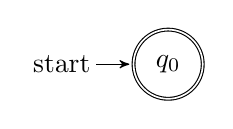
\begin{tikzpicture}[->,>=stealth',shorten >=1pt,auto,node
  distance=1cm,inner sep=2pt,
  mystate/.style={state,text centered}]

  \node[initial,accepting,mystate] (q0) {\(q_0\)};

\end{tikzpicture}
\end{document}
